%\documentclass[12pt]{article} %% required

%% style for page

\documentclass[letterpaper,12pt]{article}
\usepackage{epsfig,colortbl}
\usepackage{amssymb}
\textwidth=6.5in
\textheight=9.5in
\topmargin=-0.75in
\oddsidemargin=0.0in
\evensidemargin=0.0in
\thispagestyle{empty} % no page numbers

\usepackage{times}
\usepackage{psfig}

%%%%% Main Body %%%%%
\begin{document} %% required

{\Large \textbf{Homework 3.0}} \hfill {\small \emph{AST 422 Spring 2007}}\\

\centerline{\psfig{file=kaz_rad.ps,width=0.75\textwidth}}

\vspace{0.5cm}
\noindent Dark Gravitational Lensing?
\begin{itemize}
\item[(a)] Assume the radio source with $S_{1.4GHz}=33$ mJy.\\
Optical  $V$ $\geq$25.0 mag (HST), and $K$ $\geq$19.0 mag.\\
Use Longair Ch 2 to estimate the dark lens' \emph{minimum} $z$.\\


\item[(b)] Lensed arc background galaxy has $V$ = 24.8 mag. 
($\lambda_V = 6000 \AA$)\\
Use Longair Ch 18 (Fig 18.8) to estimate its \emph{maximum} $z$.\\
Hint: Lynman break occures at $\lambda_{L_{\alpha}}=1216 \AA$ at $z=0$.\\

\item[(c)] Use Longair Ch 4.3.4 to estimate the mass inside the 
Einstein Radius of the dark lens.\\
Remember you can use the Ned Wright's Cosmology Calculator:\\
http://www.astro.ucla.edu/~wright/CosmoCalc.html


\end{itemize}


\end{document} %% required
